\documentclass[../revisedmain.tex]{subfiles}
\begin{document}
The disc method is a way to calculate the volume (yes volume, not area) of a cylindrical object. We do not know the volume formula for an odd graph like this:
\begin{center}
	\begin{tikzpicture}
	\begin{axis}[
	colormap/cool,
	view={15}{30}]    
	
	\def\generatrix{(((2*x^4)/27) - ((4*x^3)/9))}
	
	\addplot3[
	surf,
	shader=faceted,
	samples=25,
	domain=0:6,
	domain y=0:2*pi,
	z buffer=sort,
	data cs=polarrad along x]
	({\generatrix},y,x);

	
	\end{axis}
	\end{tikzpicture}
\end{center}
But we can try and approximate it. Just like how we can use rectangles to approximate 2-d area, we can use cylinders to approximate cylindrical shapes. If we can find the two-dimensional cross-section of a revolved shape, we can calculate the volume of the revolved shape by taking an infinite sum of infinitely small discs knowing their radius (height in 2-dimensions). This means that we can find a Riemann-style rectangle in a cross-section like this:
\begin{center}
	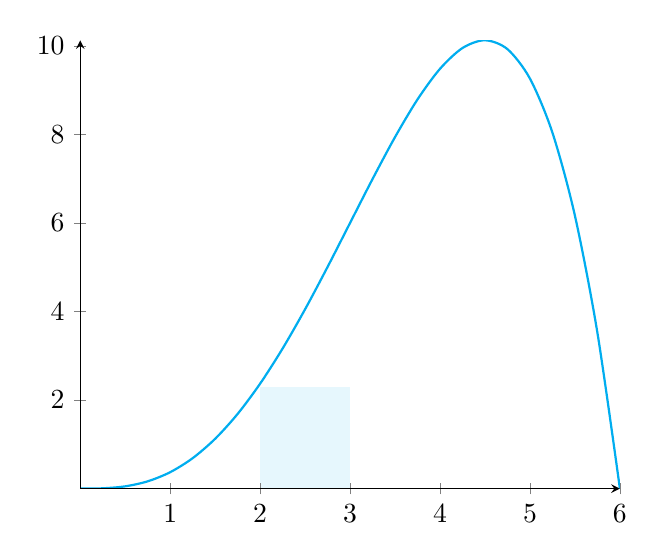
\begin{tikzpicture}
		\begin{axis}[axis lines=middle,axis on top]
		\addplot[color=cyan,smooth,thick,domain=0:6]{-(((2*x^4)/27) - ((4*x^3)/9))};
		\fill [cyan!10] (axis cs:2,0) rectangle (axis cs:3,2.3);
		\end{axis}
	\end{tikzpicture}
\end{center}
...and revolve it around the $x$-axis to create a cylinder. We can revolve infinitely small cylinders over the axis just like taking the integral. In fact, the volume of a cylinder is just $r^2 * \pi *$ height. Because we have the rectangle, we know $r=f(x)$ and height=$dx$, so we end up with a formula for revolving a cross-section about the $x$-axis:$$\pi\int_{a}^{b}f(x)^2dx$$ And if it is hollow (there is a smaller function $g(x)$ that forms the inside of the cross section, the area is $$\pi\int_{a}^{b}f(x)^2dx-\pi\int_{a}^{b}g(x)^2dx$$$$=\pi\int_{a}^{b}\left(f(x)^2-g(x)^2\right)dx$$ An easier way to remember this is big radius R minus small radius r:$$\pi\int_{a}^{b}\left(R^2-r^2\right)dx$$ or, in this case, $$\pi\int_{0}^{6}f(x)^2dx$$
\end{document}